%%-----------------------------------------

%% Vorlesungsmitschrift (Kapitel 4)

%% an der Uni Regensburg, gelesen von Christian Back

%%-----------------------------------------


\chapter{Elektromagnetische Wellen an Grenzflächen}
\section{Randbedingungen der elektromagnetischen Welle}
Wir wollen jetzt Wellenausbreitung in inhomogenen Medien beschreiben, z.B. den Übergang von Medium 1 nach Medium 2, also einer Grenzfläche.
\paragraph{Randbedingungen der MWGl.:} Die Tangentialkomponenten von $\vecE$ und $\vecH=\fracone{\muo\mu_r}\vecB$ sind stetig. Die Normalkomponenten von $\vecD=\epso\eps_r\vecE$ und $\vecB$ sind ebenfalls stetig. (isotrope, isolierende, nicht magnetische Medien $\mu=1$)
\paragraph{einfachster Fall:}zwei homogene Medien mit Brechungsindex $n_e$ (einfallender Strahl) und $n_t$ (transmittierte Welle).
%
%Skizze zu Reflexion
%
 Der Winkel $\alpha$ liegt zwischen $\veck_e$ und $\vece_y$ bzw. zwischen $\veck_t$ und $\vece_y$. Wir nehmen an, dass es eine fest vrogegebene einlaufende Welle ist.
 \begin{align*}
 	\vecE_e&=\vecE_{e_0}cor(\omega_et-\veck_e\vecr)=\vecE_{e_0}(\phi_e(\vecr,t))\\
	\vecE_r&=\vecE_{r_0}cor(\omega_rt-\veck_r\vecr+\varphi_r)=\vecE_{r_0}(\phi_r(\vecr,t))\\
	\vecE_t&=\vecE_{t_0}cor(\omega_tt-\veck_t\vecr+\varphi_t)=\vecE_{t_0}(\phi_t(\vecr,t))
 \end{align*}
 Die Wellenvektoren $\veck_e,\veck_r$ und $\veck_t$ müssen die Dispersionsrelationen im jeweiligen Medium erfüllen. Die Phasenfaktoren $\varphi_r,\varphi_t$ bestimmen die Phasenlage relativ zur einlaufenden Welle.
 %-----------------------------
 %Vorlesung vom 2.11 fehlt hier
 %-----------------------------
 
 \begin{itemize}
 	\item Wenn Licht von optisch dichteren in ein optisch dünneres Medium übergeht, ist der Reflexionskoeffizient größer null.
 	Daraus folgt, dass $\vecE_{0e}$ und $\vecE_{0e}$ in die gleiche Richtung zeigen und die Wellen an der Grenzschicht in Phase sind.
 	\item Wenn licht aus optisch dünneren in ein optisch dichteres Medium übergeht, wird der Reflexionskoeffizient kleiner Null und $\vecE_{or}$ und $\vecE_{0e}$ zeigen in antiparallele Richtungen. Außerdem liegt bei der Reflexion ein Phasensprung von $\pi$ vor, aber bei Transmission liegt kein Phasensprung vor.
 \end{itemize}
 Da die reflektierte Intensität nur proportional zu $\vert\vecE\vert^2$ ist, spielt der Phasenfaktor also keine Rolle.
 \minisec{Reflexionsgrad\nomenclature{R}{Reflexionsgrad}\index{Reflexionsgrad} der Intensität}
 \begin{align*}
 	R&= \frac{I_r}{I_e}=\left(\frac{n_e-n_t}{n_e+n_t}\right)^2=\left(\frac{n_{et}-1}{n_{et}+1}\right)^2=\left(\frac{1-n_{te}}{1+n_{te}}\right)^2
 \end{align*}
 Der Reflexionsgrad ist unabhängig von welcher Seite das Licht einfällt, sondern er hängt nur von der Änderung des relativen Brechungsindex ab. Falls das Licht aber absorbiert wird, wird der Reflexionskoeffizient komplex und kann geschrieben werden als:
 \begin{align*}
 	R=\vert r\vert^2=rr^*
 \end{align*}
 \paragraph{Beispiel:} 
 \begin{tabular}{lll}
 	Übergang&Brechungsindex&Reflexion in\%\\
 	Luft --Glas&1,5&4\%\\
 	Luft -- Diamant&2,41&17\%
 \end{tabular}
 
 \subsection{Beliebige Einfallswinkel $\alpha$}
 Zunächst betrachten wir ein $\vecE$-Feld, das parallel zur Einfallsebene schwingt und p-polarisiert (parallel zur Einfallebene) ist. Im Folgenden werden die Tangentialkomponenten mit dem Index T versehen und die Normalkomponenten mit dem Index N. Betrachte außerdem noch die Setigkeitsbedingungen für $\vecE$ und $\vecD=\epso\eps\vecE$.
 \begin{align*}
 	E_{eN}&=E_e\sin\alpha&E_{tN}&=E_t\sin\beta&E_{rN}&=E_r\sin\alpha\\
 	E_{eT}&=E_e\cos\alpha&E_{tT}&=E_t\cos\beta&E_{rT}&=-E_r\cos\alpha
 \end{align*}
 %-----------------------------------------------------------------------------------
 % Hab mir hier die Herleitung gespart oder sollen wir sie doch noch mit rein nehmen?
 %----------------------------------------------------------------------------------
 Mit Hilfe der Stetigkeitsbedingungen und der Snellschen Formel, erhalten wir daraus die \emph{Fresnelschen Formeln}\index{Fresnelsche Formeln}. Wobei $r_p$ der Reflexionskoeffizient für p-polarisiertes Licht ist.
 \begin{align}
 	r_{\parallel}&=r_p=\frac{n_t\cos\alpha -n_e\cos\beta}{n_t\cos\alpha +n_e\cos\beta}=\frac{\tan(\alpha -\beta)}{\tan(\alpha +\beta)}\label{FF1}\\
 	r_{\bot}&=r_s=\frac{n_e\cos\alpha -n_t\cos\beta}{n_e\cos\alpha +n_t\cos\beta}=-\frac{\sin(\alpha -\beta)}{\sin(\alpha +\beta)}\label{FF2}
 \end{align}
 Die Amplituden der reflektierten $\vecE$-Felder erhält man durch Multiplikation der Amplituden des emittierten $\vecE$-Felder mit den Reflexionskoeffizienten.
 \minisec{Transmittierte Leistung $P_t$\nomenclature{P_t}{transmittierte Leistung}\index{transmittierte Leistung} und Intensität $I_t$ \nomenclature{I_t}{transmittierte Intensität}\index{transmittierte Intensität}}
 Wenn man nun nicht direkt an den Amplituden, sondern nur an der Leistung interessiert ist, kann man diese auch über den Transmissionsgrad $T^P$ ( bzw. bei der Intensität $T^{I}$\index{Transmissionsgrad}\nomenclature{T^P}{Transmissionsgrad der Leistung}\nomenclature{T^I}{Transmissionsgrad der Intensität}) berechnen. Aufgrund der Energieerhaltung gilt $ P_e=P_r+P_t$ und man erhält folgende Gleichungen:
 \begin{align*}
 	T_{\parallel}^P&= 1-\vert r_{\parallel}\vert^2\\
 	T_{\bot}^P&= 1-\vert r_{\bot}\vert^2\\
 	\text{wobei:}\quad T^p&=\frac{P_t}{P_e}
 \end{align*}
 Für die Berechnung der Intensität ist allerdings die Änderung der Fläche zu berücksichtigen, da sich die Ausdehnung des Lichtstrahls auf der Einfallebene und im transmittierten Strahl ändert. 
 \begin{align*}
 d\prime&=\frac{d}{\cos\alpha}&d_t&=d\prime\cos\beta 	
 \end{align*}
 Nun kann man folgende Gleichungen formulieren.
 \begin{align*}
 	T^p&=\frac{P_t}{P_e}=\frac{I_t A_t}{I_e A}=\frac{I_t \cos\beta}{I_e\cos\alpha}=\frac{n_t\vert t\vert^2\cos\beta}{n_e\cos\alpha}\\
 	T^{I}&=\frac{I_t}{I_e}=T^P\frac{\cos\alpha}{\cos\beta}=\vert t\vert^2\frac{n_t}{n_e}
 \end{align*}
 
 \subsubsection{Diskussion der Fresnel'schen Formeln: Reflexionsgrad bei Lichteinfall aus einem optisch dünnerem Medium}
 Beispielsweise von Luft in Gas mit $\frac{n_t}{n_e}=1,5$.
 Betrachte nun die Winkelabhängigkeit von $R=\vert r\vert^2$ aus den Fresnelschen Formeln \ref{FF1} und \ref{FF2}. Bei Erhöhung des Winkels steigt $R_{\bot}$ stetig von 4\% bis 100\% an. $R_{\parallel}$ sinkt hingegen anfangs bis zu einem gewissen Winkel auf Null ab. Dieser Winkel wird auch Brewsterwinkel\index{Brewsterwinkel} genannt, danach steigt $R_{\parallel}$ ebenfalls auf die 100\% an (siehe Abb.\ref{RefGrad}).
 \begin{figure}
 	 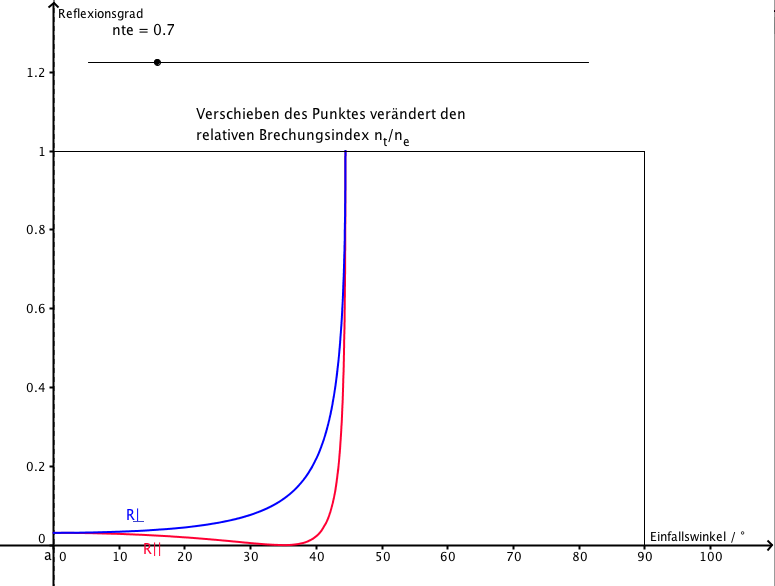
\includegraphics[width=.5\linewidth]{Bilder/Reflexionsgrad}
 	 \caption{Reflexionsgrad in Abhängigkeit des Einfallwinkels\label{RefGrad}}
 \end{figure}
Der Brewsterwinkel $\alpha_B$ oder auch $\alpha_P$ wird dann erreicht, wenn der Nenner divergiert, also $\tan(\alpha_B+\beta)=\infty$ bzw. $\alpha+\beta=90\degree$. In diesem Fall stehen der reflektierte und der gebrochene Strahl aufeinander senkrecht!  Dies lässt sich wie folgt erklären. Man nehme an, dass der reflektierte Strahl durch einen oszillierenden Dipol mit Dipolmoment parallel zum $\vecE$-Feld in der Grenzschicht erzeugt wird. Dabei ist die abgestrahlte Leistung $P(\theta)\propto\sin^2\theta$ und $\theta$ ist der Winkel zwischen Wellenvektor des abgestrahlten Lichts und  Dipolachse. Also wird längs zur Dipolachse ( $\theta=0$) kein Licht abgestrahlt -- $\vecE_{\parallel}$ wird nicht reflektiert. Daraus kann man folgern, dass das Licht vollständig linear polarisiert ist!
\begin{align*}
	\tan\alpha_B&= \frac{n_t}{n_e}
\end{align*}
 
 %
 %Vorlesung vom 9.11
 %
 
 \subsection{Absorbierende Medien}
 \begin{itemize}
 	\item Das Reflexionsvermögen bei absorbierenden Medien ist mit Fresnelformeln ebenfalls berechenbar. Man ersetze nur $n --> n_R+in_I$ mit $n_R-ik$. Nun erhält man einen komplexen Reflexionskoeffizient und Reflexionsgrad.
 	\begin{align*}
 		r&=\frac{n_{rel}-1}{n_{rel}+1}\\
 		R&=rr^*=\frac{(n_R-1)^2+n_I^2}{(n_R+1)^2+n_I^2}
 	\end{align*}
 	Das Reflexionsvermögen nimmt mit steigender Absorption zu. (z.\,B. ideal leitende Metalle $\omega<\omega_p$) Bei Spiegeln ist beispielsweise $R\approx100\%$ im Infrarot (IR), Nahinfrarot (NIR) und im sichtabren Bereich (VIS), wobei $R$ im sichtbaren Breich bereits zurück geht.
 	\item Mit wachsender Absorbtion ($n_I$ bzw. $k$) verschwindet der Brewsterwinkel, es bleibt ein Minimum von $R_{\parallel}$
 	\item Die Farbe von Gegenständen hängt von den dielektrischen Eigenschaften ab.
 \end{itemize}
 \paragraph{Annahme:}Nun wird wird im sichtbaren Bereich ein weißes Licht mit allen Spektralanteilen verwendet, um verschiedene Gegenstände zu beleuchten.
 \begin{enumerate}
 	\item \emph{Metalle} sind durch ihre hohe Leitfähigkeit charakterisiert, die sich in einer spektral breitbandigen Reflexion äußern. Dadurch entsteht der metallische Glanz.
 	\item \emph{Isolatoren, die im VIS-Bereich keine Absorption besitzen,} sind transparent. Allerdings wenn ihre Oberfläche gestört wird, werden sie weiß aufgrund ihres wellenlängenunabhänigem Reflexionsvermögen (vgl. Zucker -- Puderzucker).
 	\item Bei \emph{Isolatoren mit nur einer schwachen Absorption }im VIS-Bereich, beobachtet man in Transmission und Reflexion jeweils andere Farben. Dies wird durch die spektrale Verteilung des transmittierten Lichts bestimmt. (vgl. verdünnte Tinte)
 	\item Bei \emph{Isolatoren mit sehr hoher Absorption}, also sehr hoher Reflexion, wird die Farbe der Transmission wieder durch den Spektralbereich mit optimaler Transparenz bestimmt.
 \end{enumerate}